\section{Diagnostic Methods Supplemental Information}

\subsection{Microwave Scattering}

\begin{figure}[]
\centering
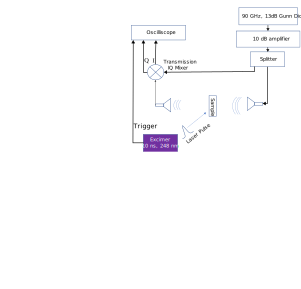
\includegraphics[width=0.8\textwidth]{\repodir/final/figures/SI/output/MWS_Setup_Silicon.png}
\caption{Microwave scattering setup for silicon wafers.}
\label{fig:SI_MWS_Setup_Silicon}
\end{figure}

\begin{figure}[]
\centering
\includegraphics[width=0.8\textwidth]{\repodir/final/dataset/output/figures/mws_nothing_T0.png}
\caption{A) Measurement of transmission without any torch, B) position dependent transmission measurement.}
\label{fig:SI_MWS}
\end{figure}

\ref{fig:SI_mws_processing_overview} shows the processing steps for the MWS data. 



\begin{figure}[]
\centering
\includegraphics[width=0.8\textwidth]{\repodir/experiment/analysis/mws/output/figures/mws_processing_overview.png}
\caption{Microwave processing overview}
\label{fig:SI_mws_processing_overview}
\end{figure}


\subsection{Laser Profile}


\begin{figure}[]
\centering
\includegraphics[width=0.8\textwidth]{\repodir/experiment/analysis/mws/output/figures/laser_profile.png}
\caption{Laser profile measurement}
\label{fig:SI_Laser_Profile}
\end{figure}